\documentclass{training}
\schoollogo{../../resources/intros/UX-02-lets-fight-harassment.jpg}
\setlang{french}
\newcommand{\uxfond}{../../resources/fond/UX-02-lets-fight-harassment.png}
% Filigrane PAR MODULE : \uxfond (PNG A4 dilue 30 %). Cadre noir vectoriel commun.
% Proportions original 744 px : marge 20/744, trait 1/744. Exterieur BLANC.
% Cadre via eso-pic +\put (coordonnees absolues) — pas de remember picture (decalage).
\usepackage{eso-pic}

\providecommand{\uxfond}{../../resources/fond/norme_fond_paliers_30.png}

\newlength{\uxmargin}
\newlength{\uxthick}
\newlength{\uxinnerw}
\newlength{\uxinnerh}
\setlength{\uxmargin}{0.02688\paperwidth}% 20/744
\setlength{\uxthick}{0.001344\paperwidth}% 1/744
\setlength{\uxinnerw}{\dimexpr\paperwidth-2\uxmargin-2\uxthick\relax}
\setlength{\uxinnerh}{\dimexpr\paperheight-2\uxmargin-2\uxthick\relax}

% Contenu strictement a l'interieur du trait (+ jour confortable).
\geometry{%
  includeheadfoot,
  left=22mm,
  right=22mm,
  top=20mm,
  bottom=18mm,
  headheight=30pt,
  headsep=5mm,
  footskip=12mm%
}

\AddToShipoutPictureBG{%
  \AtPageLowerLeft{%
    % Fond blanc page entiere
    \put(0,0){\color{white}\rule{\paperwidth}{\paperheight}}%
    % Filigrane module a l'interieur du cadre
    \put(\LenToUnit{\dimexpr\uxmargin+\uxthick\relax},\LenToUnit{\dimexpr\uxmargin+\uxthick\relax}){%
      \includegraphics[width=\uxinnerw,height=\uxinnerh]{\uxfond}}%
    % Cadre noir : bas, haut, gauche, droite
    \put(\LenToUnit{\uxmargin},\LenToUnit{\uxmargin}){%
      \color{black}\rule{\dimexpr\paperwidth-2\uxmargin\relax}{\uxthick}}%
    \put(\LenToUnit{\uxmargin},\LenToUnit{\dimexpr\paperheight-\uxmargin-\uxthick\relax}){%
      \color{black}\rule{\dimexpr\paperwidth-2\uxmargin\relax}{\uxthick}}%
    \put(\LenToUnit{\uxmargin},\LenToUnit{\uxmargin}){%
      \color{black}\rule{\uxthick}{\dimexpr\paperheight-2\uxmargin\relax}}%
    \put(\LenToUnit{\dimexpr\paperwidth-\uxmargin-\uxthick\relax},\LenToUnit{\uxmargin}){%
      \color{black}\rule{\uxthick}{\dimexpr\paperheight-2\uxmargin\relax}}%
  }%
}

\makeatletter
\fancyhf{}
\fancyheadoffset{0pt}
\renewcommand{\headrulewidth}{0pt}
\lhead{\parbox[t]{0.56\textwidth}{\RaggedRight\footnotesize\sloppy\@title}}
\rhead{\parbox[t]{0.36\textwidth}{\RaggedLeft\footnotesize\sloppy\@subtitle}}
\cfoot{\thepage}
% Coupures : underscore et slash dans les noms de fichiers / consignes
\DeclareRobustCommand{\_}{\textunderscore\allowbreak}
\makeatother

% Evite les depassements de longues lignes (Github, Name_FirstName_...)
\sloppy
\emergencystretch=3em
\hbadness=10000

% Sommaire type 42 : chapitres seulement
\setcounter{tocdepth}{0}
\renewcommand{\cftchappresnum}{}
\renewcommand{\cftchapaftersnum}{}
\setlength{\cftchapnumwidth}{2.0em}
\setlength{\cftbeforechapskip}{0.35em}
\cftsetindents{chapter}{0em}{2.0em}


\begin{document}

\title{Luttons contre le harcèlement}
\subtitle{Piscine UX/UI --- UX}
\member{Piscine UX/UI}{https://github.com/01-edu/UX-UI}
\summary{Une recherche et un message public. Le sujet n'est pas un script.}
\version{1.0}
\prerequisite{Le module précédent de cette piscine, ou aucun si c'est le premier.}
\maketitle

\newpage
\tableofcontents
\newpage


\chapter{Instructions}

L'avant-propos n'est pas un exercice. Il ne sera pas noté. Les exercices commencent au chapitre suivant, du contrat le plus simple au plus dur. Un exercice plus tardif n'est pas pris en compte si un plus tôt ne tient pas.

On ne regarde que ce qui est dans le répertoire de rendu de l'exercice. N'ajoutez pas un fichier que l'exercice ne nomme pas. Le nom d'un livrable suit le motif imprimé dans l'exercice : \texttt{Name\_FirstName\_DeliverableName\_Date\_VersionNumber}.

Le geste ne vous est pas donné. Les exemples d'un exercice portent parfois une contrainte que la phrase ne répète pas. Lisez-les. Vos autres références sont le manuel de l'outil choisi, la personne assise à côté, et les liens imprimés dans l'exercice.

L'ordre est celui de la quête. Sauter une étape parce qu'un écran plus tard semble plus intéressant produit un écran que personne ne sait expliquer.

\subsection*{Des images}

La marque en couverture est l'image de ce module. Les paliers pâles derrière le texte sont le fond de page. Ni l'un ni l'autre n'est un indice.

\subsection*{Des machines qui écrivent}

Vous pouvez vous servir d'un outil pour vérifier un mot, comme d'un dictionnaire. Vous ne pouvez pas remplacer un entretien, un test ou un fichier par un texte généré et le signer. Si vous ne pouvez pas montrer la personne, l'écran ou la ligne que vous avancez, l'exercice n'est pas fait.


\chapter{Avant-propos}

Une affiche est une phrase qu'une rue peut lire. A.~M.~Cassandre traitait l'affiche comme une voix publique, pas comme un ornement (les affiches réunies par le MoMA, \url{https://www.moma.org/artists/1015}). Cette quête demande ce genre de voix : un message pour un public réel. Elle ne demande pas de montrer le mal, et elle ne donne pas le message.

\begin{center}
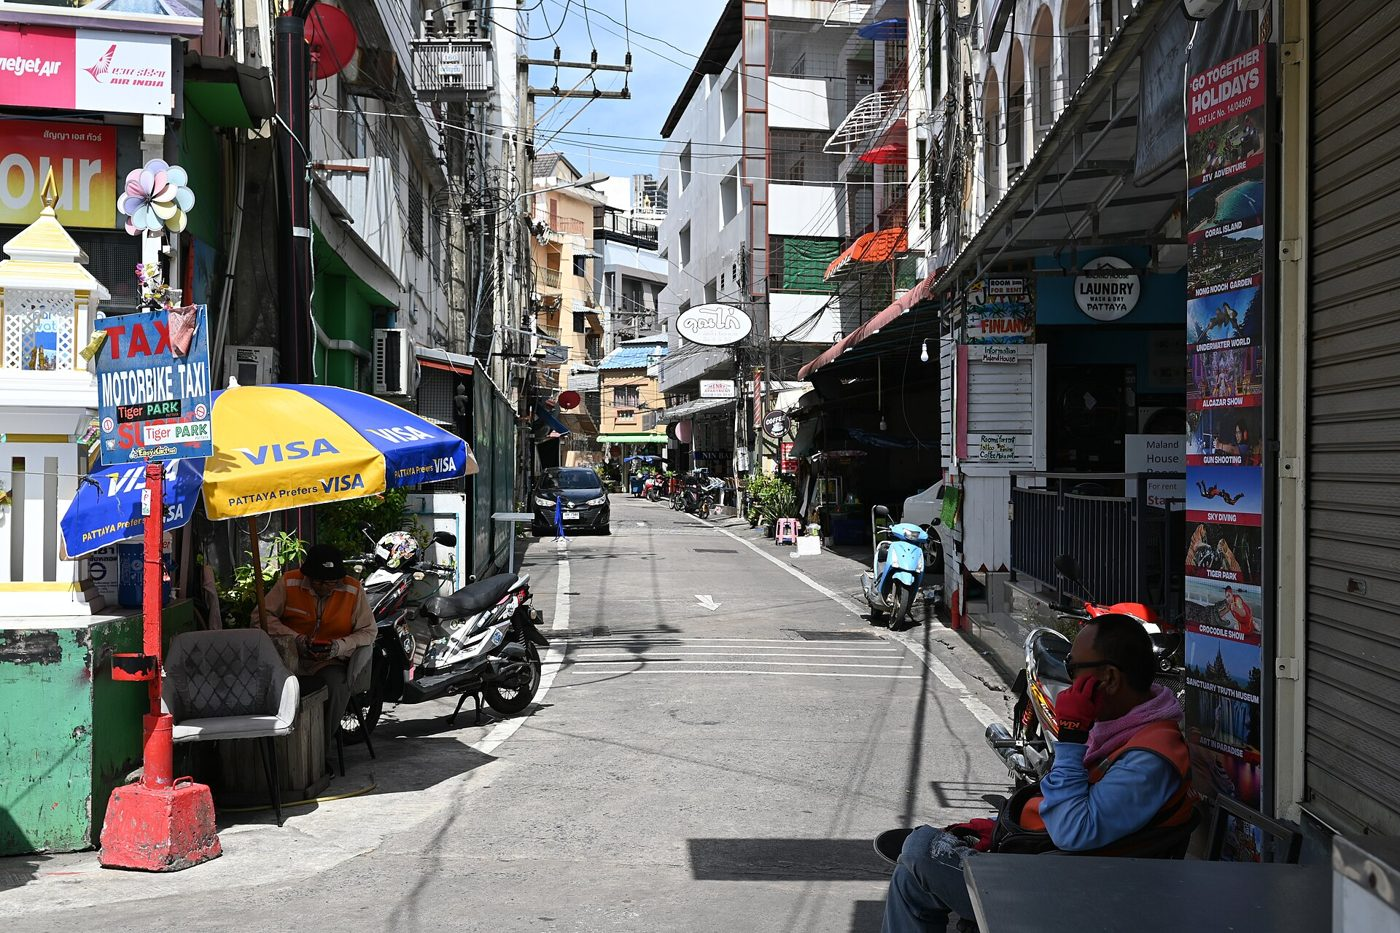
\includegraphics[width=0.78\textwidth,height=0.32\textheight,keepaspectratio]{../../resources/intros/UX-02-lets-fight-harassment.jpg}\\[0.4em]
{\footnotesize Image : PattayaPatrol, CC BY-SA 4.0}
\end{center}

À regarder. Les vidéos sont un contexte. Elles ne sont pas le livrable.
\begin{itemize}
\item UX - Introduction \& Quest n°1, 01Edu \url{https://www.youtube.com/watch?v=UbE6WMeuvQg&list=PLHyAJ_GrRtf-RAtfngbRrFh1XDTnyXFDe}
\end{itemize}

\chapter{Exercice 00 : UX III - Ex 1 - Analyse concurrentielle}
\exnumber{00}
\extitle{UX III - Ex 1 - Analyse concurrentielle}
\exfiles{ex00/archive zip, nomme Name\_FirstName\_DeliverableName\_Date\_VersionNumber}
\exauthorize{Ceux nommés dans l'exercice}
\makeheaderfiles

\textbf{Contexte :}

La quête n°3 porte sur l'Empathie.

Dans ce scénario, le principal de votre lycée a appris que vous étiez designer. Il a choisi de faire appel à vous pour l'aider à faire face au harcèlement scolaire parmi les adolescents.

Le harcèlement scolaire décrit des comportements de harcèlement en milieu scolaire. Il se caractérise par l'usage répété de violence, y compris la moquerie et d'autres humiliations.

En fait, ils se sont rendu compte qu'ils ne connaissaient pas très bien cette génération (15 à 18 ans). Ils vous demandent donc de mener une recherche utilisateur pour rencontrer cette population et la comprendre.

Votre travail est d'explorer votre sujet et d'utiliser divers outils inclus dans cette phase « Empathize ».

\textbf{Instructions :}

Menez une analyse concurrentielle parmi 10 associations ou organisations luttant contre le harcèlement scolaire.

Vous pouvez choisir 10 organisations dans le monde, ou de votre région ou de votre pays d'origine. Naviguons !

Comparez les actions principales, canaux et valeurs de ces 10 organisations, selon les critères que vous jugez pertinents.

\textbf{Livrables :}

\begin{itemize}
\item Un rapport concurrentiel avec une introduction qui explique vos conclusions principales (PDF)
\item Un graphique pour montrer le paysage concurrentiel, avec 2 axes de votre choix (numérique, psychologique, local, proximité des étudiants, institutionnel, etc.) (PDF)
\item Un tableau pour comparer les organisations sur 5 à 10 critères (PDF)
\item Déposez les documents sur Github, dans un zip nommé « ProjectTitle\_Name\_FirstName », et chaque livrable ainsi : « Name\_FirstName\_DeliverableName\_Date\_VersionNumber ». Exemple : « Doe\_John\_MidFiPrototype\_05242024\_V1 ».
\item Ajoutez un titre dans tous les documents écrits.
\item Soignez l'aspect global des livrables. Ils doivent être clairs, simples et lisibles. Vous pouvez regarder canva.com, sans surcharger le dessin de détails.
\end{itemize}

Ressources :

\begin{itemize}
\item Analyse concurrentielle : comment l'aborder efficacement \url{https://uxdesign.cc/competitive-analysis-how-to-approach-it-effectively-def97d130d2c}
\item Templates d'analyse concurrentielle \url{https://venngage.com/blog/competitor-analysis-template/}
\end{itemize}

\textbf{Citation :}

\begin{itemize}
\item « Concevez toujours une chose dans son contexte plus large : une chaise dans une pièce, une pièce dans une maison, une maison dans un environnement, un environnement dans un plan urbain » Eero Sarrinen | Knoll
\item Créer un grand design ne consiste pas seulement à comprendre ce que l'utilisateur veut. Il s'agit aussi de comprendre et de répondre aux besoins de l'entreprise.
\end{itemize}


\chapter{Exercice 01 : UX III - Ex 2 - Questionnaires}
\exnumber{01}
\extitle{UX III - Ex 2 - Questionnaires}
\exfiles{ex01/PDF, nomme Name\_FirstName\_DeliverableName\_Date\_VersionNumber}
\exauthorize{Ceux nommés dans l'exercice}
\makeheaderfiles

\textbf{Instructions :}

Préparez un questionnaire pour collecter des données quantitatives auprès de vos utilisateurs.

Et rappelez-vous, vous n'êtes pas votre utilisateur !

Pour être utilisé dans des études sérieuses et obtenir des résultats viables, un formulaire doit recueillir au moins 100 réponses. Les réponses doivent vous donner des données quantifiables que vous pouvez utiliser pour prouver un point et confirmer des tendances, pas des verbatims ou des détails.

\textbf{Livrables :}

\begin{itemize}
\item Un document PDF comprenant votre ou vos objectif(s) et vos hypothèses, les questions, une introduction et une conclusion.
\item Dans le document, ajouter le lien vers un questionnaire prêt à être diffusé
\item Déposez le PDF sur Github, nommé ainsi : « Name\_FirstName\_DeliverableName\_Date\_VersionNumber ». Exemple : « Doe\_John\_MidFiPrototype\_05242024\_V1 ».
\item Ajoutez un titre dans le document.
\item Soignez l'aspect global du document. Il doit être clair, simple et lisible. Vous pouvez regarder canva.com, sans surcharger le dessin de détails.
\end{itemize}

\textbf{Pistes :}

Voici les étapes recommandées :

1. Définissez votre objectif, ce que vous cherchez en diffusant votre formulaire aux gens. Habituellement, cela concerne des chiffres, des proportions, etc.
2. Notez 1 à 3 hypothèses que vous avez sur ce sujet, que vous devez soit confirmer soit infirmer.
3. Choisissez 3 à 5 sujets sur lesquels il vous faut de l'information.
4. Pour chaque sujet, rédigez 1 à 3 questions fermées. Rappelez-vous, votre utilisateur doit répondre par un choix dans une liste de réponses préparées ou utiliser l'option « autre » pour écrire la réponse qu'il ne trouve pas dans la liste préparée.
5. Rédigez quelques questions de screening pour obtenir quelques données démographiques (âge, métier, localisation, etc.). Cela vous permet de vous assurer que les réponses obtenues viennent de votre cible.
6. Structurez vos questions en entonnoir : commencez par des questions larges pour vous concentrer sur des sujets ou situations spécifiques. N'oubliez pas de rester neutre dans votre ton pour laisser l'utilisateur raconter sa propre histoire. Essayez de vous concentrer sur 10 questions principales.
7. Rédigez une introduction de salutation, décrivant brièvement (1) qui vous êtes et (2) ce que vous cherchez. Pas besoin d'en dire trop, mais assez pour fournir un cadre et l'objectif du formulaire.
8. Rédigez une conclusion pour remercier votre utilisateur pour son temps, et préparez les prochaines étapes. Ex. : demander de diffuser ce formulaire à 3 personnes, etc.

\textbf{Obligatoire : demandez-leur s'ils seraient disponibles pour un entretien anonyme en personne (par téléphone, en présentiel, en visioconférence : selon ce qui les met le plus à l'aise), car vous devrez mener au moins 3 entretiens par la suite.}

\textbf{Ressources :}

\begin{itemize}
\item Lean Survey Canvas : comment l'utiliser \url{https://medium.com/think-big-work-smart/the-lean-survey-canvas-1b0a00cab200}
\item Questionnaires utilisateurs - Comment interroger vos utilisateurs \url{https://refiner.io/blog/user-surveys/}
\item Concevoir un excellent questionnaire en 3 étapes simples \url{https://uxdesign.cc/designing-a-great-survey-with-3-simple-steps-283abaa67ad6}
\item Questionnaires UX : un guide rapide pour en tirer le meilleur \url{https://uxdesign.cc/ux-surveys-a-quick-guide-to-get-the-most-out-of-them-1889d136be6a}
\item Mieux rechercher grâce aux questionnaires \url{https://uxmastery.com/better-user-research-through-surveys/}
\item L'expérience utilisateur des questionnaires \url{https://uxdesign.cc/the-user-experience-of-surveys-a5420c82604a}
\end{itemize}

\textbf{Outils :}

\begin{itemize}
\item Typeform \url{https://www.typeform.com/}
\item Google Forms \url{https://docs.google.com/forms/u/0/}
\end{itemize}

\textbf{Citations :}

\begin{itemize}
\item « Les questionnaires mesurent et catégorisent les attitudes ou collectent des données autodéclarées qui peuvent aider à suivre ou découvrir des problèmes importants à traiter. » Norman Nielsen Group
\item Les questionnaires ne sont pas précis pour fournir des données comportementales car LES UTILISATEURS OMETTENT DES ÉTAPES AU MILIEU ET LES SOUVENIRS SONT DÉFAILLANTS.
\end{itemize}


\chapter{Exercice 02 : UX III - Ex 3 - Stratégie de diffusion}
\exnumber{02}
\extitle{UX III - Ex 3 - Stratégie de diffusion}
\exfiles{ex02/archive zip, nomme Name\_FirstName\_DeliverableName\_Date\_VersionNumber}
\exauthorize{Those named in the exercise}
\makeheaderfiles

\textbf{Instructions :}

Define and run your broadcast strategy among teenagers (15-18 years old)

Even though a proper survey requires at least 100 answers, for this exercise we request you to get 40.

\textbf{Livrables :}

\begin{itemize}
\item A PDF document gathering your strategy. Please include:
\begin{itemize}
\item Who you are targeting (remember, you can focus on your hometown as well as the whole planet)
\item A few ideas about how to reach them
\item The channels you intend to use - be specific and include the links to the groups, forums, pages, account you plan to reach
\item At least 2 different messages
\item A plan A, a plan B, a plan C
\end{itemize}
\item A document to express your main feedback after running your broadcast strategy: what worked best? have you encountered any difficulties? What were they? How did you overcome them?
\item Déposez les documents sur Github, dans un zip nommé « ProjectTitle\_Name\_FirstName », et chaque livrable ainsi : « Name\_FirstName\_DeliverableName\_Date\_VersionNumber ». Exemple : « Doe\_John\_MidFiPrototype\_05242024\_V1 ».
\item Ajoutez un titre dans tous les documents écrits.
\item Soignez l'aspect global des livrables. Ils doivent être clairs, simples et lisibles. Vous pouvez regarder canva.com, sans surcharger le dessin de détails.
\end{itemize}

\textbf{Pistes :}

In order to do so, you need to be creative and strategic!

\begin{itemize}
\item Who are you targeting? Teenagers, bullies, persecutor, witnesses, parents, teachers, people in the administration? From where?
\item How can you reach them? Through which channels? On which forums, groups, with which hashtags? Will you try to get them through influencers?
\item What words and what tone will you use?
\item How will you approach them? What message will you write?
\item What have you planned if they don't answer right away?
\end{itemize}

Once your strategy is prepared, run it!

\textbf{Resource:}

\begin{itemize}
\item How to get more survey responses \url{https://rafflepress.com/how-to-get-more-survey-responses/}
\end{itemize}


\chapter{Exercice 03 : UX III - Ex 4 - Entretiens}
\exnumber{03}
\extitle{UX III - Ex 4 - Entretiens}
\exfiles{ex03/fichier Figma et PDF, nomme Name\_FirstName\_DeliverableName\_Date\_VersionNumber}
\exauthorize{Those named in the exercise}
\makeheaderfiles

\textbf{Instructions :}

\begin{itemize}
\item Create an interview guide
\item Conduct 3 interviews with teenagers
\end{itemize}

After knowing more about trends and "What" people do thanks to surveys, the main goal is to understand "why".

\textbf{Livrables :}

\begin{itemize}
\item A PDF document with an interview guide
\item A PDF document with 3 scripts 
\item An affinity diagram from your interviews (PDF or digital, on Miro or Figma for example)
\item Déposez les documents sur Github, dans un zip nommé « ProjectTitle\_Name\_FirstName », et chaque livrable ainsi : « Name\_FirstName\_DeliverableName\_Date\_VersionNumber ». Exemple : « Doe\_John\_MidFiPrototype\_05242024\_V1 ».
\item Ajoutez un titre dans tous les documents écrits.
\item Soignez l'aspect global des livrables. Ils doivent être clairs, simples et lisibles. Vous pouvez regarder canva.com, sans surcharger le dessin de détails.
\end{itemize}

\textbf{Ressources :}

\begin{itemize}
\item Respondent - Tool to find users \url{https://www.respondent.io}
\item How to conduct user interviews \url{https://uxdesign.cc/how-to-conduct-user-interviews-fe4b8c34b0b7?sk=9625632a522a9309a91297191e668565}
\item How to design better products through user interviews \url{https://uxdesign.cc/how-to-design-better-products-through-user-interviews-4c5142bb1fc4}
\item Asking the right questions \url{https://uxdesign.cc/asking-the-right-questions-on-user-research-interviews-and-testing-427261742a67}
\end{itemize}

\textbf{Pistes :}

Voici les étapes recommandées :

1. Define your objective, what you are looking for when interviewing people. Usually, this has to do with your user's habits, and the most painful problems they have regarding this topic.
2. Write down 1 to 3 hypotheses you have regarding this topic, that needs to be either confirmed or disproved.
3. Choisissez 3 à 5 sujets sur lesquels il vous faut de l'information.
4. For each topic, write 1 to 3 open-ended questions. Remember, your user cannot answer with "Yes" or "No"! Ex: How, Why, What, When, Tell me about the last time you did... etc. If you really need to introduce a new topic by a close-ended question, ask why right after.
5. Write some screening questions to have a few pieces of demographics (age, job, location, etc.)
6. Structure your questions in a funnel: start with broad questions to focus on specific topics or situation. Remember to stay neutral in your tone to let the user tell their own story. Try to focus on 10 main questions.
7. Write a greeting introduction, describing briefly (1) who you are and (2) what you are looking for. No need to say too much, but enough to provide a framework and the purpose of the interview.
8. Write a conclusion to thank your user for their time, and prepare the next steps. Ex: ask to be put in touch with someone they know and who could be interested in this topic, etc.


\chapter{Exercice 04 : UX III - Ex 5 - Personas}
\exnumber{04}
\extitle{UX III - Ex 5 - Personas}
\exfiles{ex04/fichier Figma et PDF, nomme Name\_FirstName\_DeliverableName\_Date\_VersionNumber}
\exauthorize{Those named in the exercise}
\makeheaderfiles

\textbf{Instructions :}

Let's create a persona based on your quantitative research and your interviews.

Your persona card should include common trends amongst the people you got data from (habits, verbatims, fears, drivers, frustration, and pain points).

Reminder: Your persona is fictional and should not have the exact name or picture as someone you interviewed, but remember a persona is here so you can make decisions as a designer.

\textbf{Livrables :}

\begin{itemize}
\item A PDF persona card extracted from a Figma file
\item Déposez le PDF sur Github, nommé ainsi : « Name\_FirstName\_DeliverableName\_Date\_VersionNumber ». Exemple : « Doe\_John\_MidFiPrototype\_05242024\_V1 ».
\item Ajoutez un titre dans le document.
\item Soignez l'aspect global du document. Il doit être clair, simple et lisible. Vous pouvez regarder canva.com, sans surcharger le dessin de détails.
\end{itemize}

\textbf{Ressources :}

\begin{itemize}
\item Make your persona great again \url{https://uxdesign.cc/personas-e60c1c06ead1}
\item Persona, journey maps, user flow, site map, OH MY! \url{https://uxdesign.cc/personas-journey-maps-site-maps-and-user-flows-oh-my-e71d044b4bcb}
\item Persona framework \url{https://miro.medium.com/max/1400/0*RbHfR6BHhhFIENNf}
\end{itemize}

\textbf{Citations :}

\begin{itemize}
\item If you design for everyone, you delight no one.
\item A good user persona is the one based on user research, without regard to how many attributes we can describe.
\end{itemize}


\chapter{Exercice 05 : UX III - Ex 6 - Parcours utilisateur}
\exnumber{05}
\extitle{UX III - Ex 6 - Parcours utilisateur}
\exfiles{ex05/fichier Figma, nomme Name\_FirstName\_DeliverableName\_Date\_VersionNumber}
\exauthorize{Those named in the exercise}
\makeheaderfiles

\textbf{Instructions :}

Now you have your persona, it's time to set it in motion.

Design a User Journey to represent your persona in their environment across the time, with key steps or actions related to our current topic (harassment).

The timeline can be of a day, a few hours, or a week. Please include the key moments related to harassment alongside the emotions related to each step. Use the material from your interviews and surveys.

Then, highlight the main pain points that need to be solved.

\textbf{Livrable :}

\begin{itemize}
\item A Figma document with your persona's user journey
\item Déposez le fichier Figma sur Github, nommé ainsi : « Name\_FirstName\_DeliverableName\_Date\_VersionNumber ». Exemple : « Doe\_John\_MidFiPrototype\_05242024\_V1 ».
\item Ajoutez un titre dans le fichier.
\item Soignez l'aspect global du fichier. Il doit être clair, simple et lisible. Vous pouvez regarder canva.com, sans surcharger le dessin de détails.
\end{itemize}

\textbf{Ressources :}

Most articles you'll find will be about user journeys or customer journeys. Keep in mind that you can adapt this methodology to any persona with any kind of situation or process, even at school, outside the school, in the digital world, etc.

\begin{itemize}
\item A Lean UX Customer Journey Map \url{https://uxdesign.cc/proto-journey-a-lean-ux-customer-journey-map-30ea3a241edc}
\item How to create a Customer Journey Map \url{https://www.youtube.com/watch?v=mSxpVRo3BLg}
\item Journey Mapping: How to build it \url{https://www.lucidchart.com/blog/how-to-build-customer-journey-maps}
\item Journey Mapping template \url{https://d2slcw3kip6qmk.cloudfront.net/marketing/blog/2017Q3/SEO-initiative-customer-journey-mapping/CustomerJourneyMap1.png}
\item Journey Mapping example on Figma \url{https://www.figma.com/file/5tittjiznRCWTNR2xI5FIT/Untitled?node-id=0%3A1}
\item Example \url{https://d2slcw3kip6qmk.cloudfront.net/marketing/blog/2017Q3/SEO-initiative-customer-journey-mapping/CustomerJourneyMap1.png}
\end{itemize}

\textbf{Citations :}

\begin{itemize}
\item "More options = More problems." Scott Belsky | VP of Product \& Community Adobe
\item 'A customer journey map is a visualization of the process that a person goes through in order to accomplish a goal. It's used for understanding and addressing customer needs and pain points' Norman Nielsen Group
\end{itemize}


\chapter{Exercice 06 : UX III - Ex 7 - Énoncé du problème}
\exnumber{06}
\extitle{UX III - Ex 7 - Énoncé du problème}
\exfiles{ex06/PDF, nomme Name\_FirstName\_DeliverableName\_Date\_VersionNumber}
\exauthorize{Those named in the exercise}
\makeheaderfiles

\textbf{Instructions :}
Based on your previous work, your persona and your user journey's main painpoint, define a problem statement that would clarify the main problem you want to tackle.
You may use the How Might We exercise in pairs.

Then, define 3 KPIs (Key performance Indicators) that will help you measure the definition of Done and the success of the solution.

\textbf{Livrables :}

\begin{itemize}
\item A PDF document with one problem statement and 3 KPIs to measure the impact of the solution
\item Déposez le PDF sur Github, nommé ainsi : « Name\_FirstName\_DeliverableName\_Date\_VersionNumber ». Exemple : « Doe\_John\_MidFiPrototype\_05242024\_V1 ».
\item Ajoutez un titre dans le document.
\item Soignez l'aspect global du document. Il doit être clair, simple et lisible. Vous pouvez regarder canva.com, sans surcharger le dessin de détails.
\end{itemize}

\textbf{Ressources :}

\begin{itemize}
\item Stuck on a problem? Just ask how might we \url{https://relab.academy/design-thinking/stuck-on-a-problem-just-ask-how-might-we/}
\item Problem statement \url{https://www.indeed.com/career-advice/career-development/what-is-a-problem-statement}
\item Using 'How Might We' Questions to Ideative on the Right Problems \url{https://www.nngroup.com/articles/how-might-we-questions/}
\item Unleashing the power of a UX KPI \url{https://articles.uie.com/power_of_ux_kpi/}
\item KPI is an imperative tool for UX designers \url{https://uxdesign.cc/kpi-is-the-most-important-tool-ux-designers-should-be-learning-to-use-af31651120fc?sk=e619213adfda152171d597fc3ab1053a}
\item Measuring product design impact  ---  KPIs, NPS, UX, WTF \url{https://uxdesign.cc/measuring-product-design-impact-kpis-nps-ux-wtf-3fe6a26e7400?sk=52c1f3842edbe90524f6da1fe85db71d}
\item A metrics-driven approach to evaluate success of UX design \url{https://uxdesign.cc/a-metrics-driven-approach-to-evaluate-success-of-ux-design-dd3bea098820?sk=acf1b1f7f0a7663d34d11906339b4698}
\item A big list of UX KPIs and metrics \url{https://www.cxpartners.co.uk/our-thinking/big_list_of_ux_kpis_and_metrics/}
\item How to use SMART goals to build your KPIs \url{https://www.grow.com/blog/how-to-use-smart-goals-to-build-your-kpis}
\item Exampels of KPIs (fake data! Not to be copied or used!): 
\begin{itemize}
\item Harassment case report rates increase by 20\% within 2 years
\item Online harassment drops by 30\% within 5 years
\item 90\% of the 15-18 year-olds knows a harassment witness response process within 2 years
\end{itemize}
\end{itemize}

\textbf{Citation :}

'Every problem is an opportunity for design. By framing your challenge as a How Might We question, you'll set yourself up for an innovative solution' IDEO


\end{document}
